\subsubsection{Communication Decryption} \label{section:counter-replace-encryption-content-communication}
The third approach is to use encryption on the server response.
This is an additional security feature which is applied in combination with a content server described in subsection~\ref{section:counter-replace-server}.
When the user does the login on the server, additional unique device specific paramters have be passed as well.
The server generates a cryptographic key which is used for communication is encrypted
\begin{figure}[h]
    \centering
    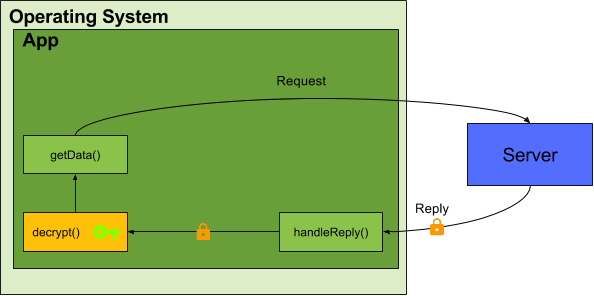
\includegraphics[width=0.8\textwidth]{data/encryptionComm.png}
    \caption{Encrypted communication with a server}
    \label{fig:encryptionComm}
\end{figure}
combined with device specific key, accounts cannot be shared anymore (either hacked or shared libratly)


\url{https://source.android.com/devices/drm.html} store key outside the app and decrypt content, works only for apps which can work with content server, focuses on the security of content on the phone\newline
delivering content is allowed but the deliverer wants to be sure that nobody steals it from the phone
